%!TEX root = ../main.tex
\appendix
\renewcommand{\thesection}{\Alph{section}}
\begin{appendices}
	\section{Screen Design}
	\label{screen_design}
	\hfill
	\begin{figure}[h!]
		\centering
		\begin{subfigure}{0.33\textwidth}  	      
			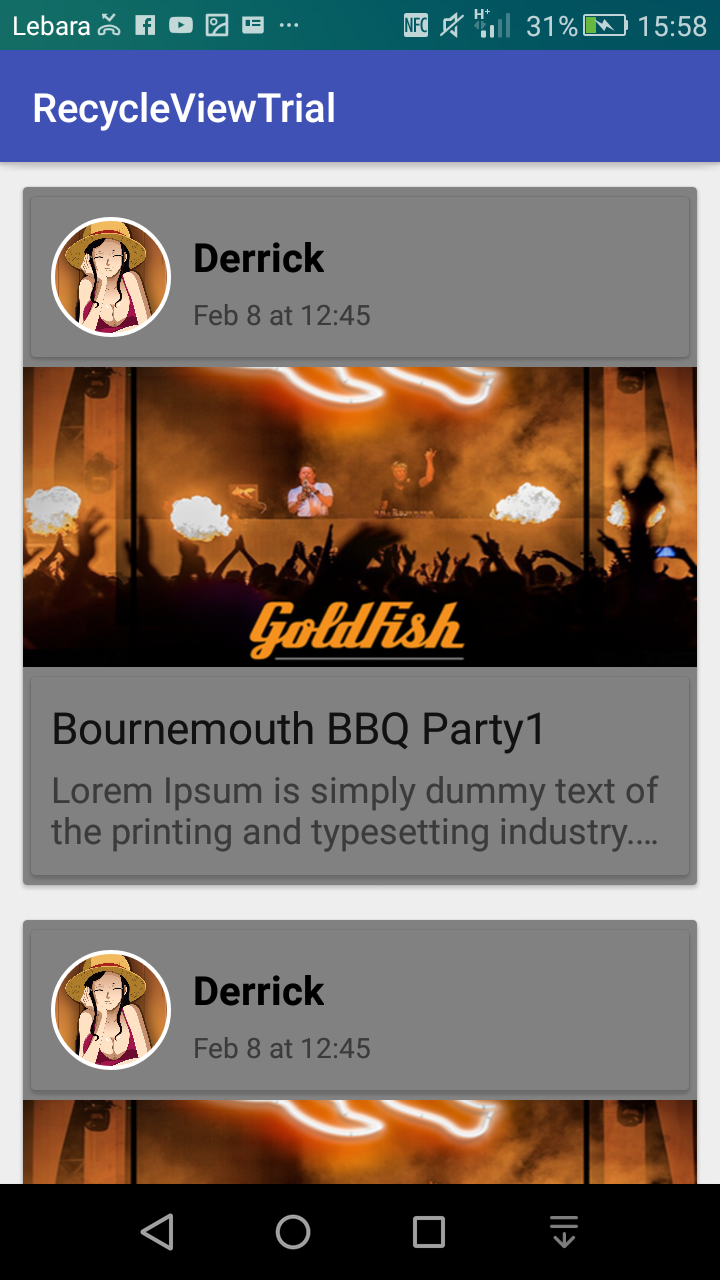
\includegraphics[width=.9\linewidth]{feed1}
		\end{subfigure}%
		%add desired spacing between images, e. g. ~, \quad, \qquad etc.
		%(or a blank line to force the subfigure onto a new line)
		\begin{subfigure}{0.30\textwidth}	
			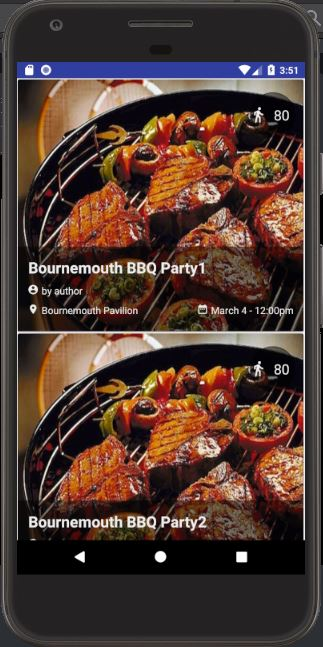
\includegraphics[width=.9\linewidth]{Feed}
			\end{subfigure}
		\begin{subfigure}{0.3\textwidth}	
		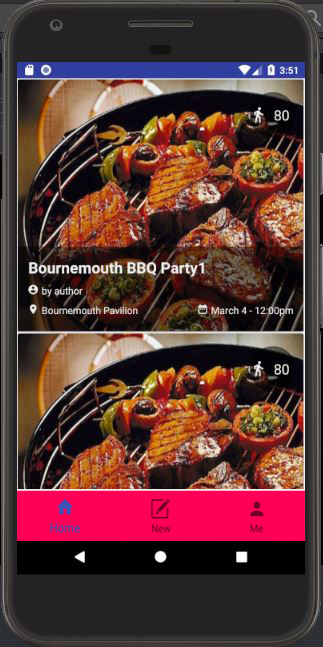
\includegraphics[width=.9\linewidth]{bottom_menu}
	\end{subfigure}
\caption{Initial Home Screen Design}
	\end{figure}
	\FloatBarrier

\begin{figure}[h!]
	\centering
	\begin{subfigure}{0.4\textwidth}
			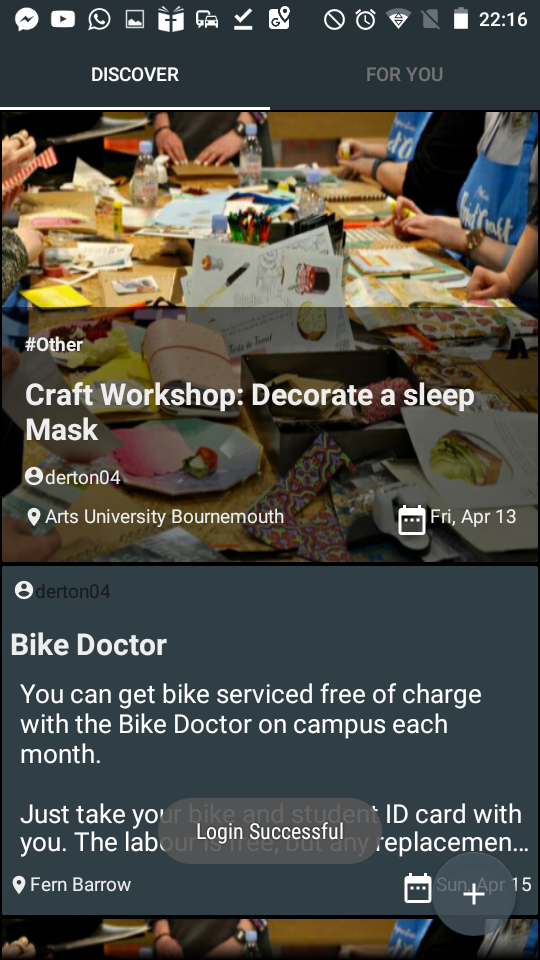
\includegraphics[width= 0.9\linewidth]{discover}
	\end{subfigure}
	\begin{subfigure}{0.4\textwidth}
	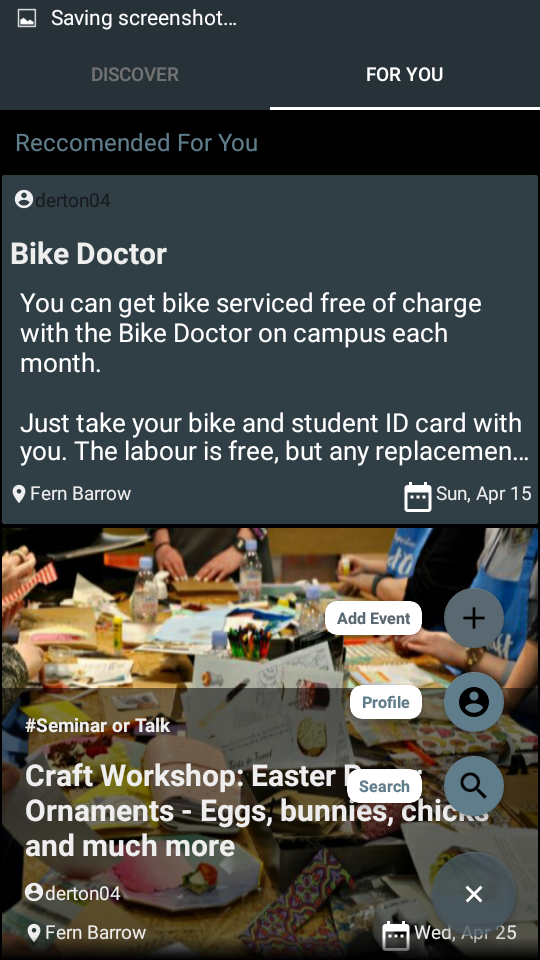
\includegraphics[width= 0.9\linewidth]{interest}
\end{subfigure}
\caption{Final Home Screen Design}
\end{figure}


	\hfill
\begin{figure}[h!]
	\centering
	\begin{subfigure}{0.30\textwidth}  	      
		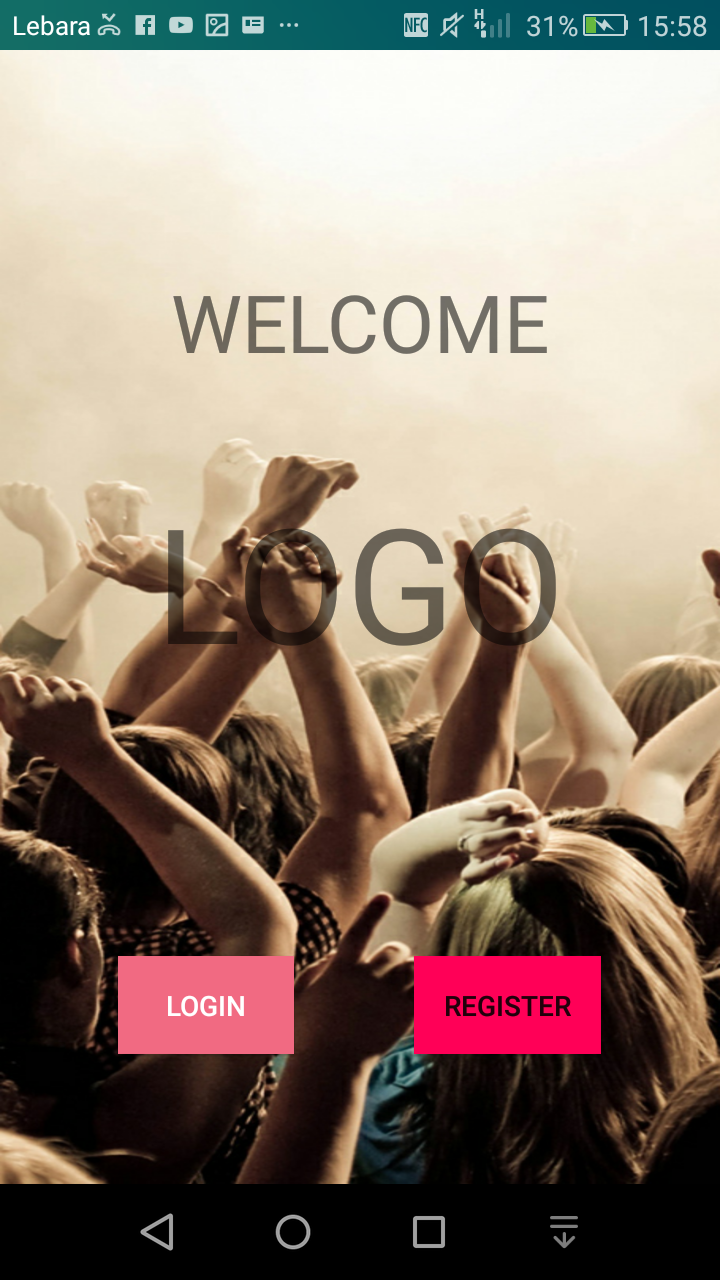
\includegraphics[width=.9\linewidth]{welcome}
	\end{subfigure}%
	%add desired spacing between images, e. g. ~, \quad, \qquad etc.
	%(or a blank line to force the subfigure onto a new line)
	\begin{subfigure}{0.30\textwidth}	
		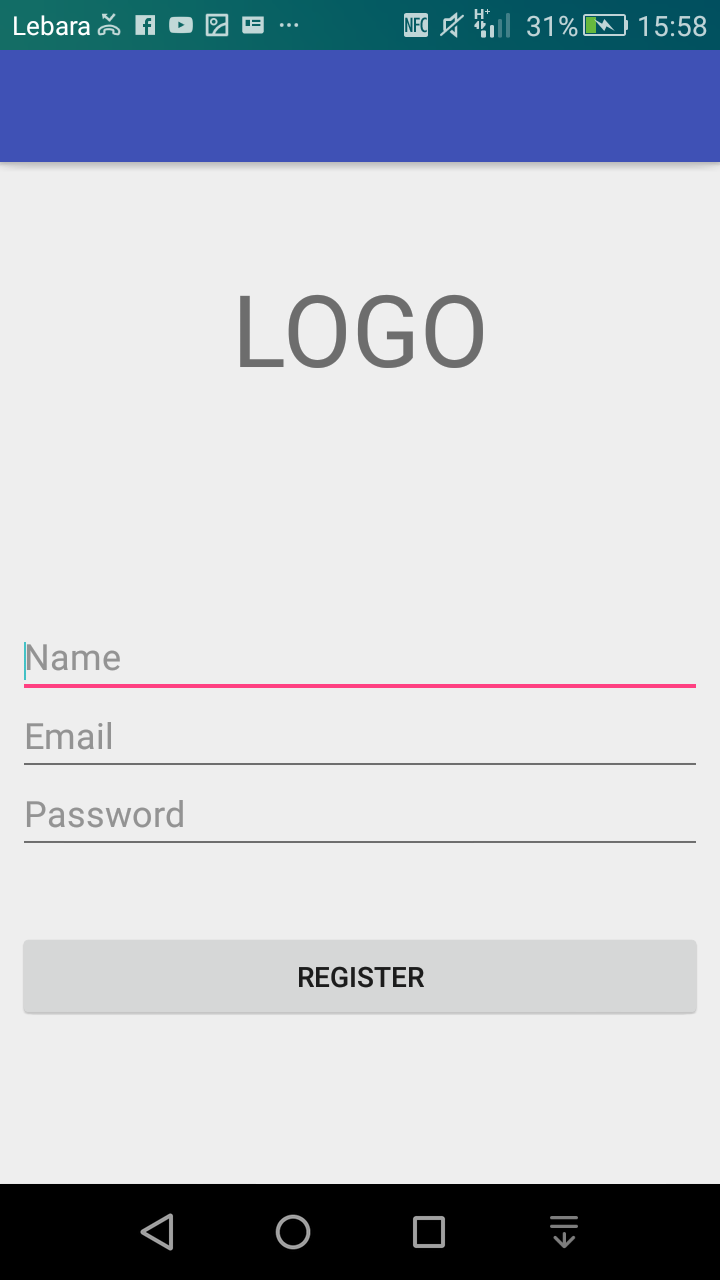
\includegraphics[width=.9\linewidth]{register_1}
	\end{subfigure}
	\begin{subfigure}{0.2\textheight}	
		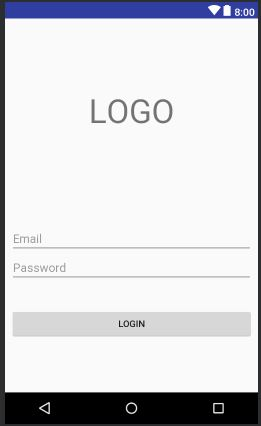
\includegraphics[width=.9\linewidth,scale=0.6]{login_1}
	\end{subfigure}
\caption{Initial Register \& Login Screen Design}
\end{figure}

\begin{figure}[h!]
	\centering
	\begin{subfigure}{0.30\textwidth}  	      
		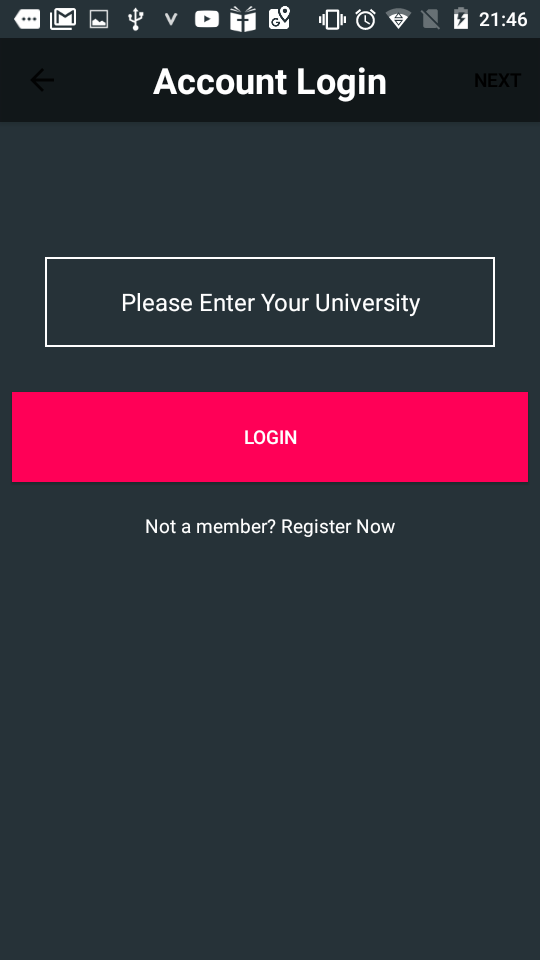
\includegraphics[width=.9\linewidth]{initial_login_screen}
	\end{subfigure}%
	%add desired spacing between images, e. g. ~, \quad, \qquad etc.
	%(or a blank line to force the subfigure onto a new line)
	\begin{subfigure}{0.30\textwidth}	
		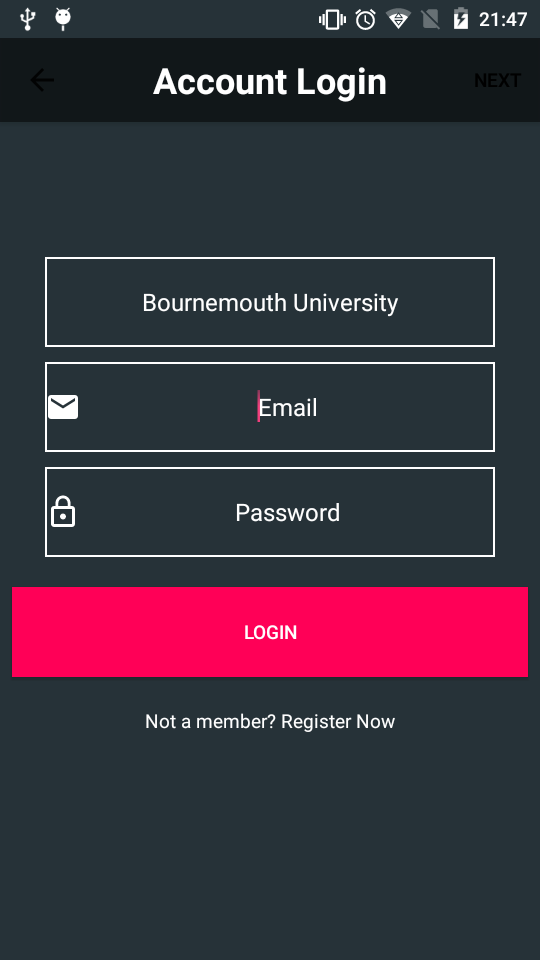
\includegraphics[width=.9\linewidth]{account_login}
	\end{subfigure}
	\begin{subfigure}{0.19\textheight}	
		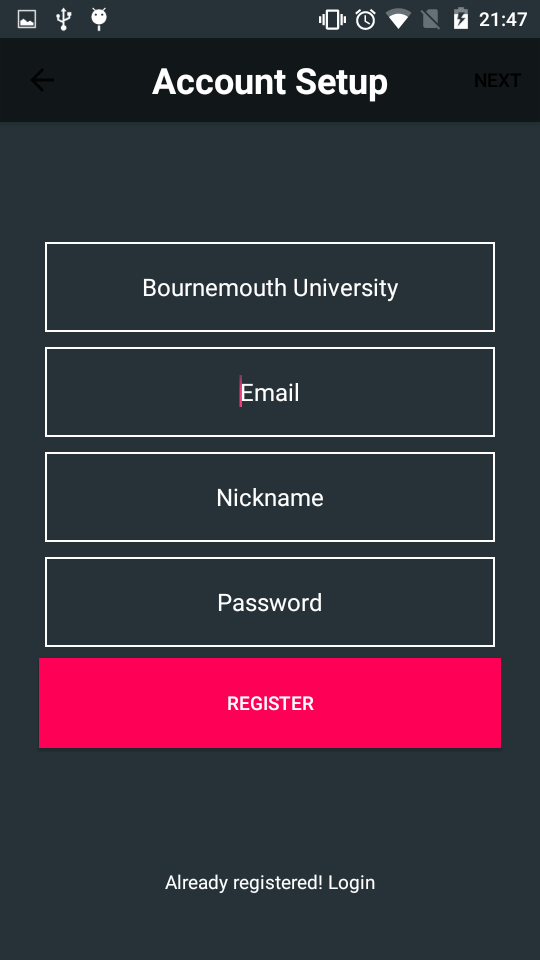
\includegraphics[width=.9\linewidth,scale=0.80]{account_Setup}
	\end{subfigure}
	\caption{Final Register \& Login Screen Design}
\end{figure}

\begin{figure}[h!]
	\centering
	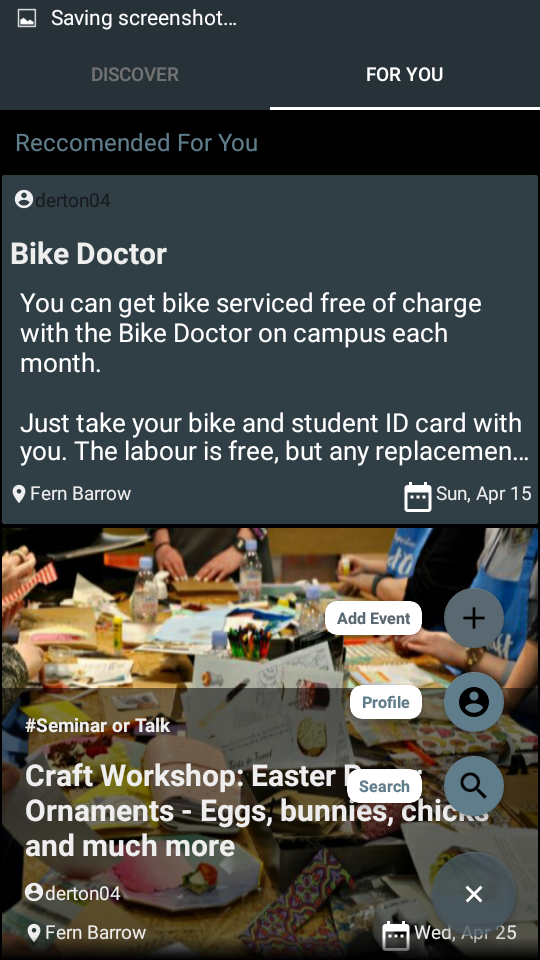
\includegraphics[width=0.2\textheight]{interest}
		\caption{Menu Clicked Screen}
\end{figure}

\begin{figure}[h!]
	\centering
	\begin{subfigure}{0.30\textwidth}  	      
		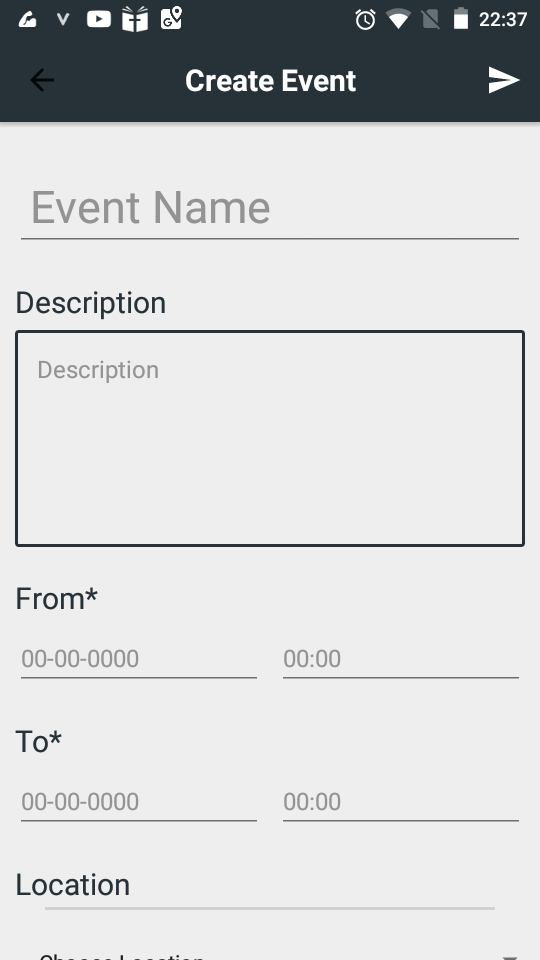
\includegraphics[width=.9\linewidth]{add_event1}
	\end{subfigure}%
	%add desired spacing between images, e. g. ~, \quad, \qquad etc.
	%(or a blank line to force the subfigure onto a new line)
	\begin{subfigure}{0.30\textwidth}	
		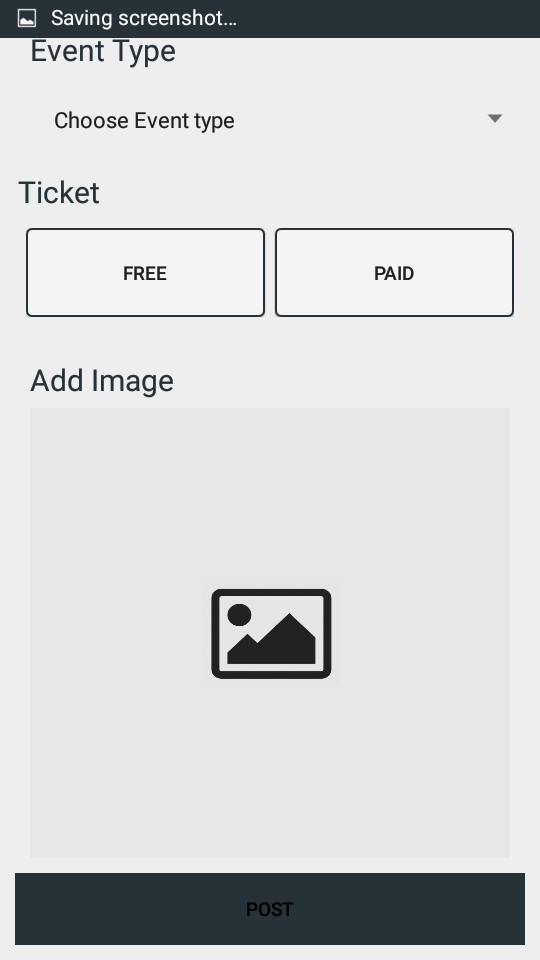
\includegraphics[width=.9\linewidth]{add_event2}
	\end{subfigure}
	\caption{Add Event Screen}
\end{figure}

\begin{figure}[h!]
	\centering
	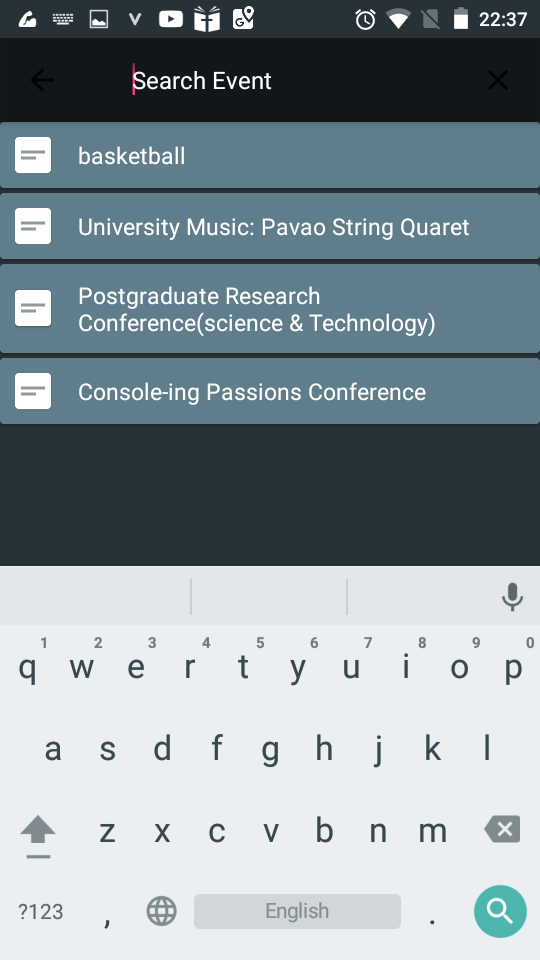
\includegraphics[width=0.2\textheight]{search}
	\caption{Search Event Screen}
\end{figure}

\begin{figure}[h!]
	\centering
	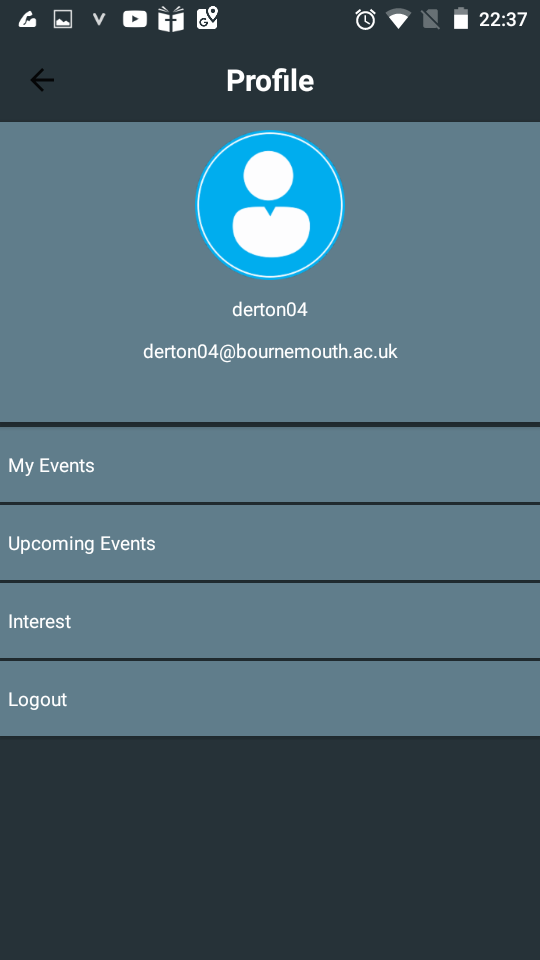
\includegraphics[width=0.2\textheight]{profile_me}
		\caption{Profile Screen}
\end{figure}

\begin{figure}[h!]
	\centering
	\begin{subfigure}{0.30\textwidth}  	      
		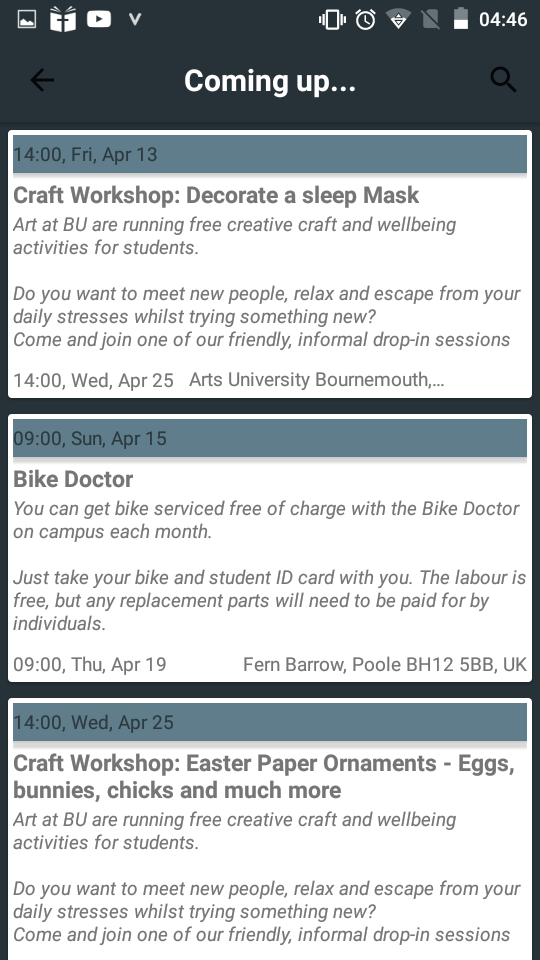
\includegraphics[width=.9\linewidth]{upcoming}
	\end{subfigure}%
	%add desired spacing between images, e. g. ~, \quad, \qquad etc.
	%(or a blank line to force the subfigure onto a new line)
	\begin{subfigure}{0.30\textwidth}	
		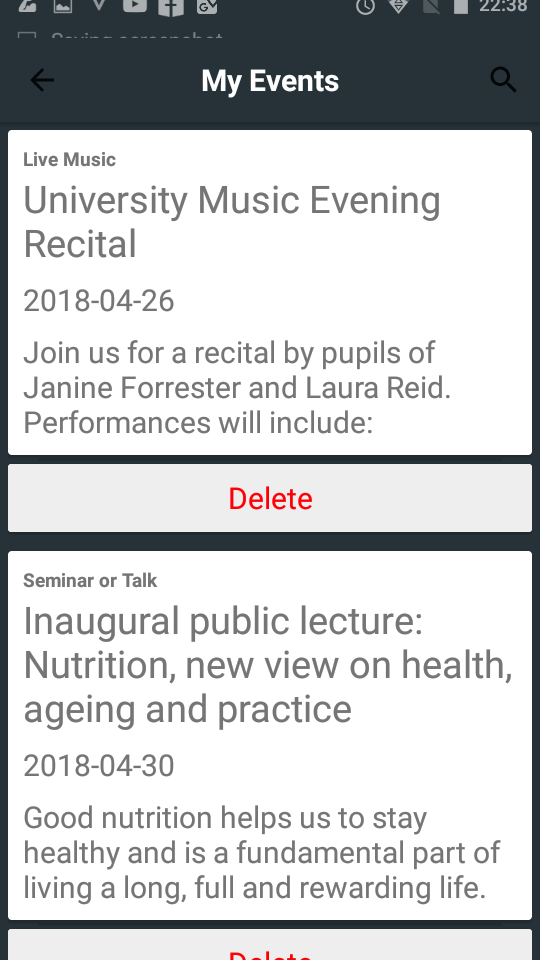
\includegraphics[width=.9\linewidth]{myevents}
	\end{subfigure}
	\begin{subfigure}{0.30\textwidth}  	      
	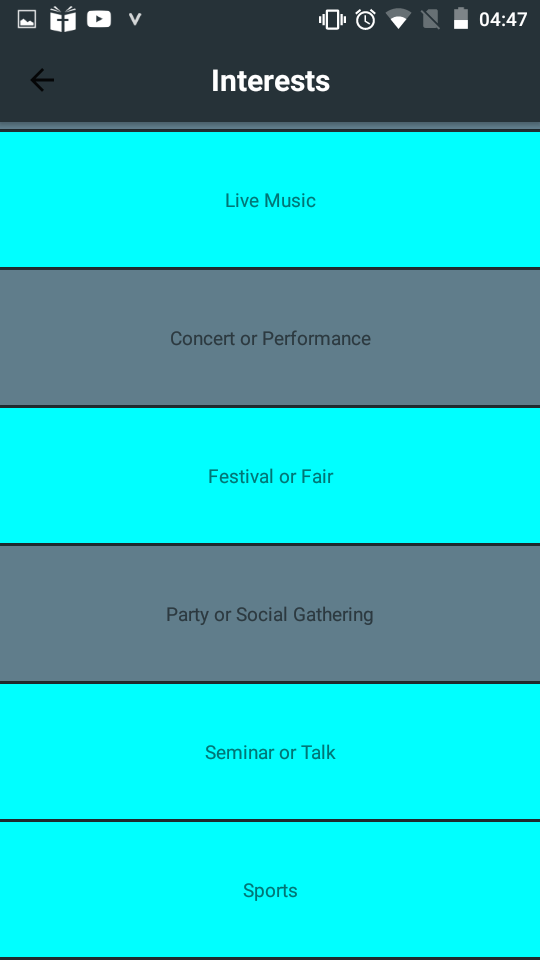
\includegraphics[width=.9\linewidth]{interest_option}
\end{subfigure}%
	\caption{Upcoming, My Events \& Choose Interest Screen}
\end{figure}



\begin{figure}[h!]
	\centering
	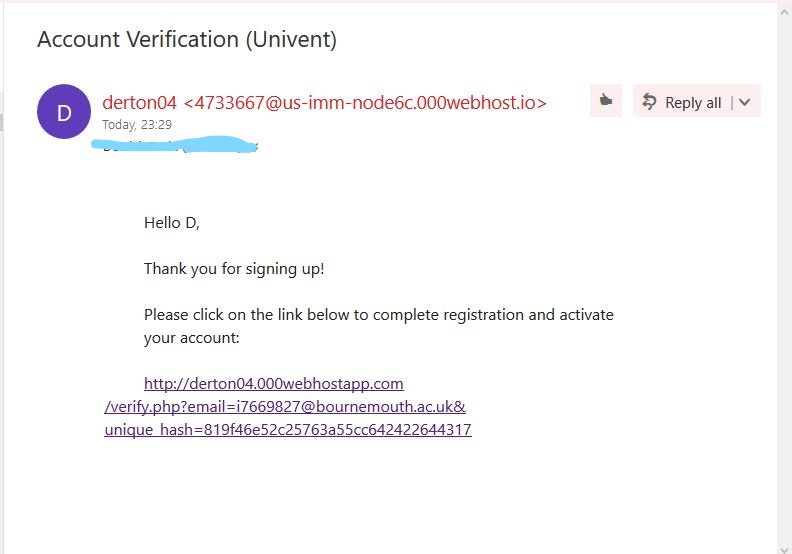
\includegraphics[width=0.4\textheight]{email_verification}
	\caption{Email Verification}
\end{figure}

\begin{figure}[h!]
	\centering
	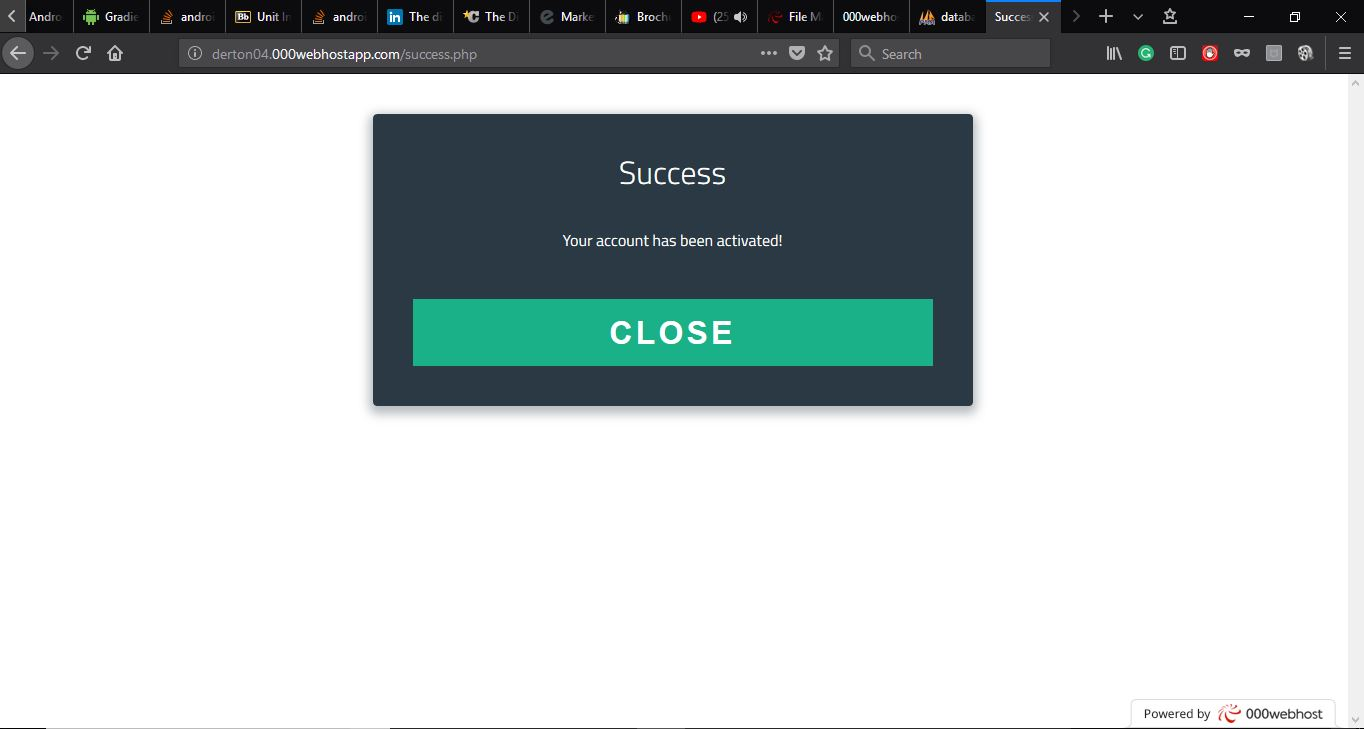
\includegraphics[width=0.4\textheight]{account_verified_Web}
	\caption{Account Verification Success}
\end{figure}

\begin{figure}[h!]
	\centering
	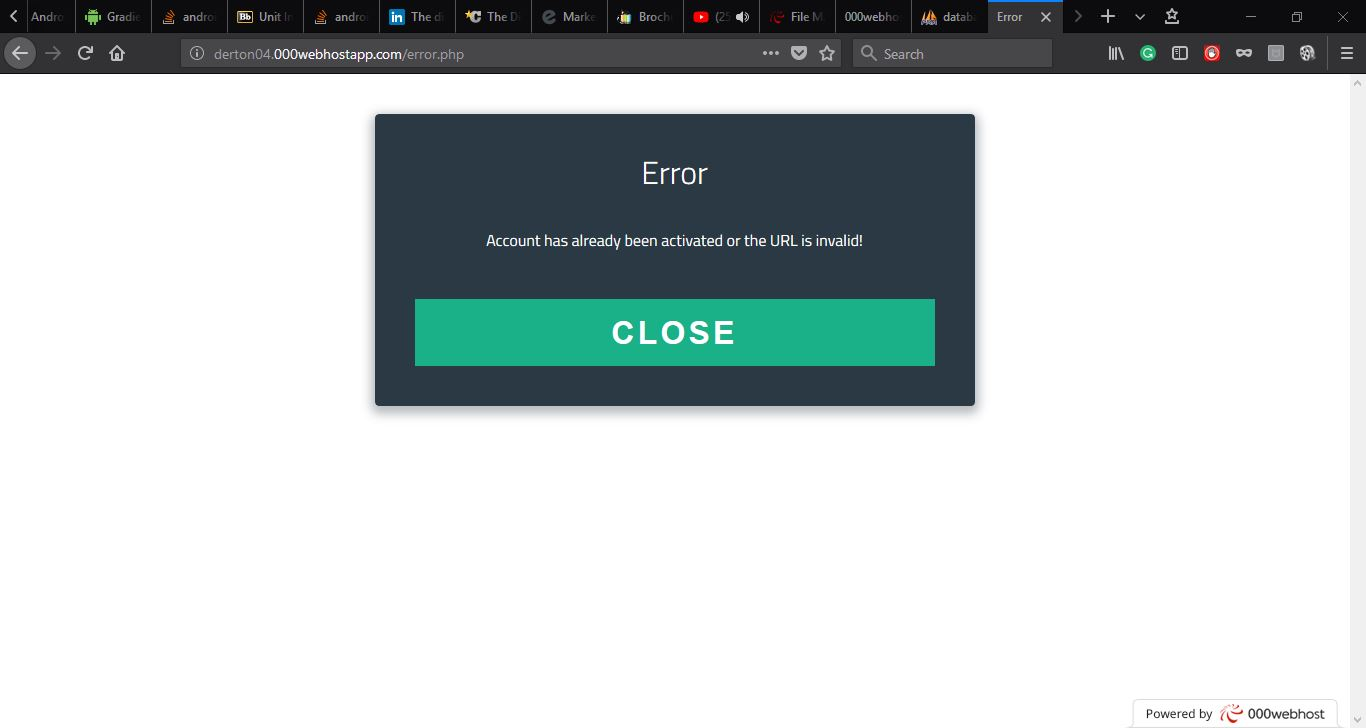
\includegraphics[width=0.4\textheight]{account_verify_error}
	\caption{Account Verification Error}
\end{figure}

\pagebreak

\section{Android vs IOS}
\label{androidvsios}
The operating system(OS) is a program that controls the execution of application and acts as an interface between a computer user and the computer hardware. The OS has these main objectives; first it has to make a computing system easy to use, secondly it has to execute programs and facilitate troubleshooting for user; and third it has to efficiently use the hardware of the computing system; \cite{stallings2001operating} cited in \cite{novac2017comparative}.

With the introduction of iOS and Android by Apple and Google, the way of thinking about operating system completely changed.
Android is by far the leading mobile platform, currently holding 86\% of the market shares against iOS holding of 12\% - 20\%.

One of the major differences between these two is the devices they run on. Android, since based on linux, runs on a variety of devices, while iOS can only run on Apple manufactured devices.

The Android OS, is an open source platform, meaning it has the ability to run third party tools, so users can add more functionality enhance performance and add more features to it, while Apple is more restricted, even though both operating systems and final products are maintained and developed by the same company. 

\begin{figure}[h]
	\centering
	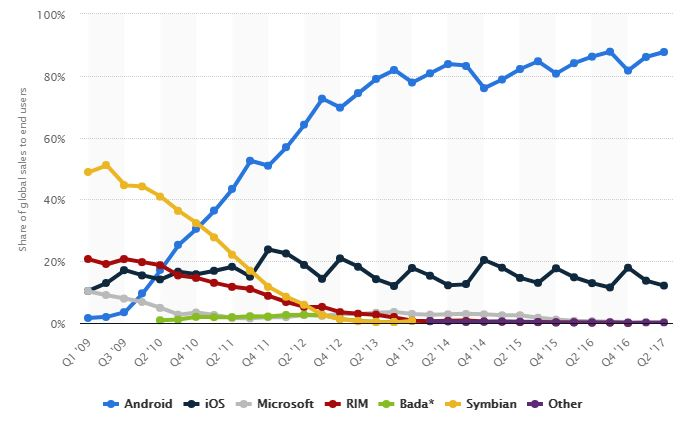
\includegraphics[width=0.6\textheight]{and_vs_ios_stat}	
	\caption{OS Global Market Share, (Data collected from Statista)}
	\label{fib:and_vs_ios_stat}
\end{figure}
The idea behind this project is to build an Android mobile application which will help people in Universities to have easy access to events activities on the faculty. Android platform was chosen, as the leading OS on the market.
\hfill
\section{JSON Data Format}
\label{json}
\begin{figure}[h!]
	\centering       
	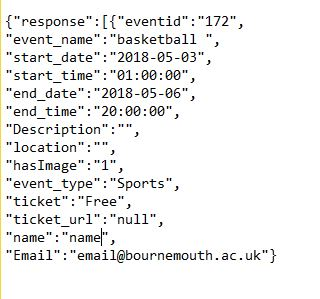
\includegraphics[scale=0.9]{json_data}
	\caption{JSON Format}
\end{figure}

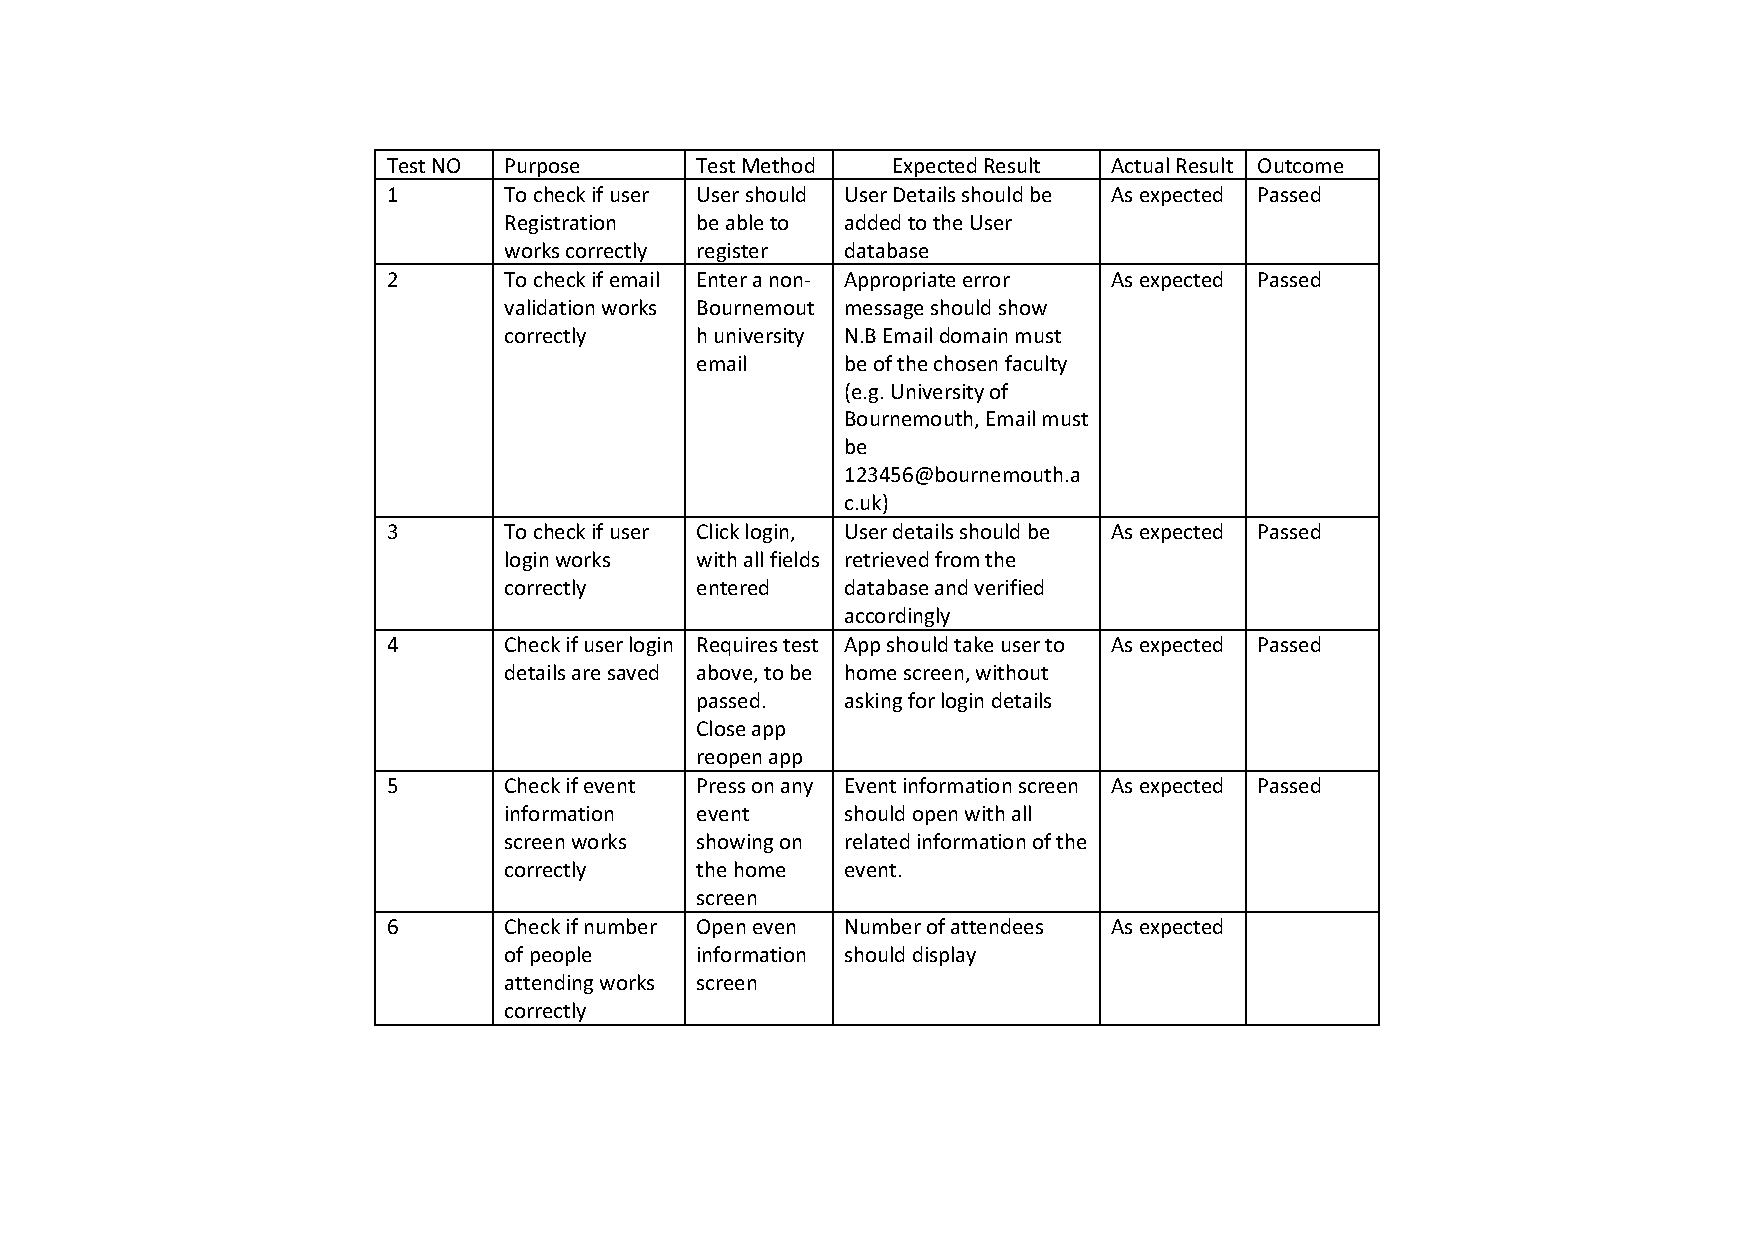
\includepdf[scale=0.85,pages=1,pagecommand=\section{Test Suit}\label{appendix:test_suit}
]{Testing}
\includepdf[pages=2-5]{Testing}

\section{Android Framework \& API}
\label{framework}
Android is built on a framework and an API. According to webopedia an API is \say{an application program interface (API), set of routines, protocols, and tools for building software applications. Basically, an API specifies how software components should interact. Additionally, APIs are used when programming graphical user interface (GUI) components. A good API makes it easier to develop a program by providing all the building blocks. A programmer then puts the blocks together}.

A framework provides an interface for Android Apps to access the
system resources. As an example, LocationManager is presented in this layer to support Android apps retrieving GPS coordinates of a device. It consists of tools for designing UIs like buttons, text fields, and system tools like intents.

\subsection{Application Component}
According to the Android developers website, application components are the essential building blocks of an Android app. Each component is an entry point through which the system or a user can enter your app.  These components are loosely coupled by the application manifest file AndroidManifest.xml that describes each component of the application and how they interact.

There are four different types of app components:
\begin{itemize}
	\item Activities.
	\item Services.
	\item Broadcast receivers.
	\item Content providers.	
\end{itemize}
Each type serves a distinct purpose and has a distinct lifecycle that defines how the component is created and destroyed. The following sections describe the four types of App components.

\subsection{Main Application Component}
\begin{itemize}
	\item \textbf{Activity} - 
	This is the visible part of the Android application, it manages the views that define what the screen looks like and how the user can interact with it. The activity has a specific life cycle as shown in figure \ref{fig:lifecycle}.
	\begin{figure}[h]
		\centering
		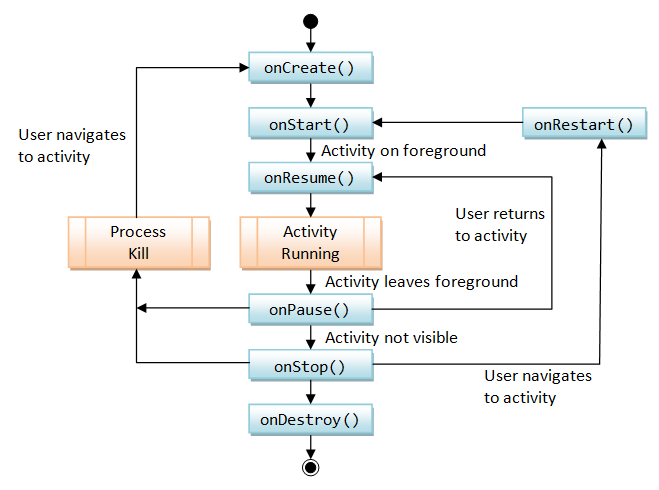
\includegraphics[width=0.5\textwidth]{Android_ActivityLifeCycle}
		\caption{Activity Lifecycle}
		\label{fig:lifecycle}
	\end{figure}
	When an activity is launched, it is brought up on the activity stack, and made visible. Oncreate, OnStart, OnResume will be called in the process. The activity from which the new activity is launched will be signalled with Onpause or OnStop. Lastly, one activity can be used to call another; a call to finish() on the  activity removes it from the stack, this is done in combination with startActivity, so the new activity will replace the current one instead of going on top of it.
	
	\item  \textbf{Service} -
	is a running component, that doesn't have an interface but has a connection with the activity. It is a component that runs in the background to perform complicated and long tasks, for example, playing music and or while continually checking for new data. 
	
	\item  \textbf{Broadcast Receivers} -
	Broadcast receivers, simply handles communication between the system and the application. For example, a broadcast announcing that the screen has turned off or the battery is low. Apps can also initiate broadcasts, for example, to let other apps know that data has been downloaded to the device and is available for them to use.
	
	\item \textbf{Content Provider} - 
	Content provider handles data sharing among applications on request or to save some data. Such requests are dealt with by methods in the content provider class.
	
\end{itemize}

\subsection{Additional Components}
\label{additional_components}
\begin{itemize}
	\item \textbf {Intent} - Most of the activities are activated by an asynchronous message called an intent.
	Intent manages interactions between application components across the whole system. They are like messengers that request an action from other components, whether the component belongs to the app or another. An interesting example is the Map application that handles Intents request to display specific GEO location. 
	
	Intent mechanism makes it easy to reuse different system components across the platform. They can
	focus on really innovative and unique functionality and simply add (’attach’) new components
	like maps or navigation to their applications which makes them even more compelling and
	useful, \cite{kwon2016design}.
	
	\item \textbf{Manifest} - 
	Every Android application has its own AndroidManifest.xml file in the root directory. This file lists all the activities and defines the properties of the application, for example the permission to the Android platform to access the internet.
\end{itemize}

\section{Sending Image to Server}
\label{sending_image_server_appendix}
This section will explain how the event images were uploaded to the server using the Volley library. 
Volley is a networking library developed by Google, easy to use, implement and memory efficient. 
It makes networking faster and easier for apps. The volley library has the features like automatic scheduling of network request, request prioritisation, cancel/block a request. Volley uses cache to improve the  performance by saving memory and bandwidth of remote server, for example, when user request the same data, instead of calling again from the server, Volley will directly load it from cache, saving resource and improving user experience.
To upload the image to the server, it has to be encoded as a base64 encoded string in android. Uploading images to server in android is time consuming process and as well as the code is also very complex. The image is converted into Base64 string format and sent to server using volley network library and the server side will decode that image through the  PHP file and finally save the image to the folder in the server(to easy fetch the image from the server, the event title is used as the image name on the server, this process of adding the image is done synchronously while uploading a new event to the database.). Uploading image as base64 reduces the time of uploading and complexity of the code.

The image is fetched from the server using the glide library. According to Github, \say{Glide is an Image Loader Library for Android developed by bumptech and is a library that is recommended by Google. It has been used in many Google open source projects including Google I/O 2014 official application. It provides animated GIF support and handles image loading/caching.}

Each image is called synchronously, while the events are being fetched from the database, as to increase performance, so the image will be displayed together with each event.
The snippet below shows how to fetch an image from the server.
\begin{figure}[h!]
	\centering       
	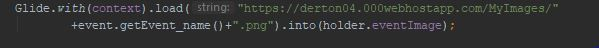
\includegraphics[width=0.5\textheight]{fetch_image}
	\caption{Glide Usage}
	\label{fig:glide_usage}	
\end{figure}
In the snippet above, https is the protocol, derton04.000webhostapp.com , the domain name, and MyImages the path where the image file is saved and event.getEvent\_name()+"png", gets the event name plus the file format png, into(holder.eventImage) is the imageView that displays the image.

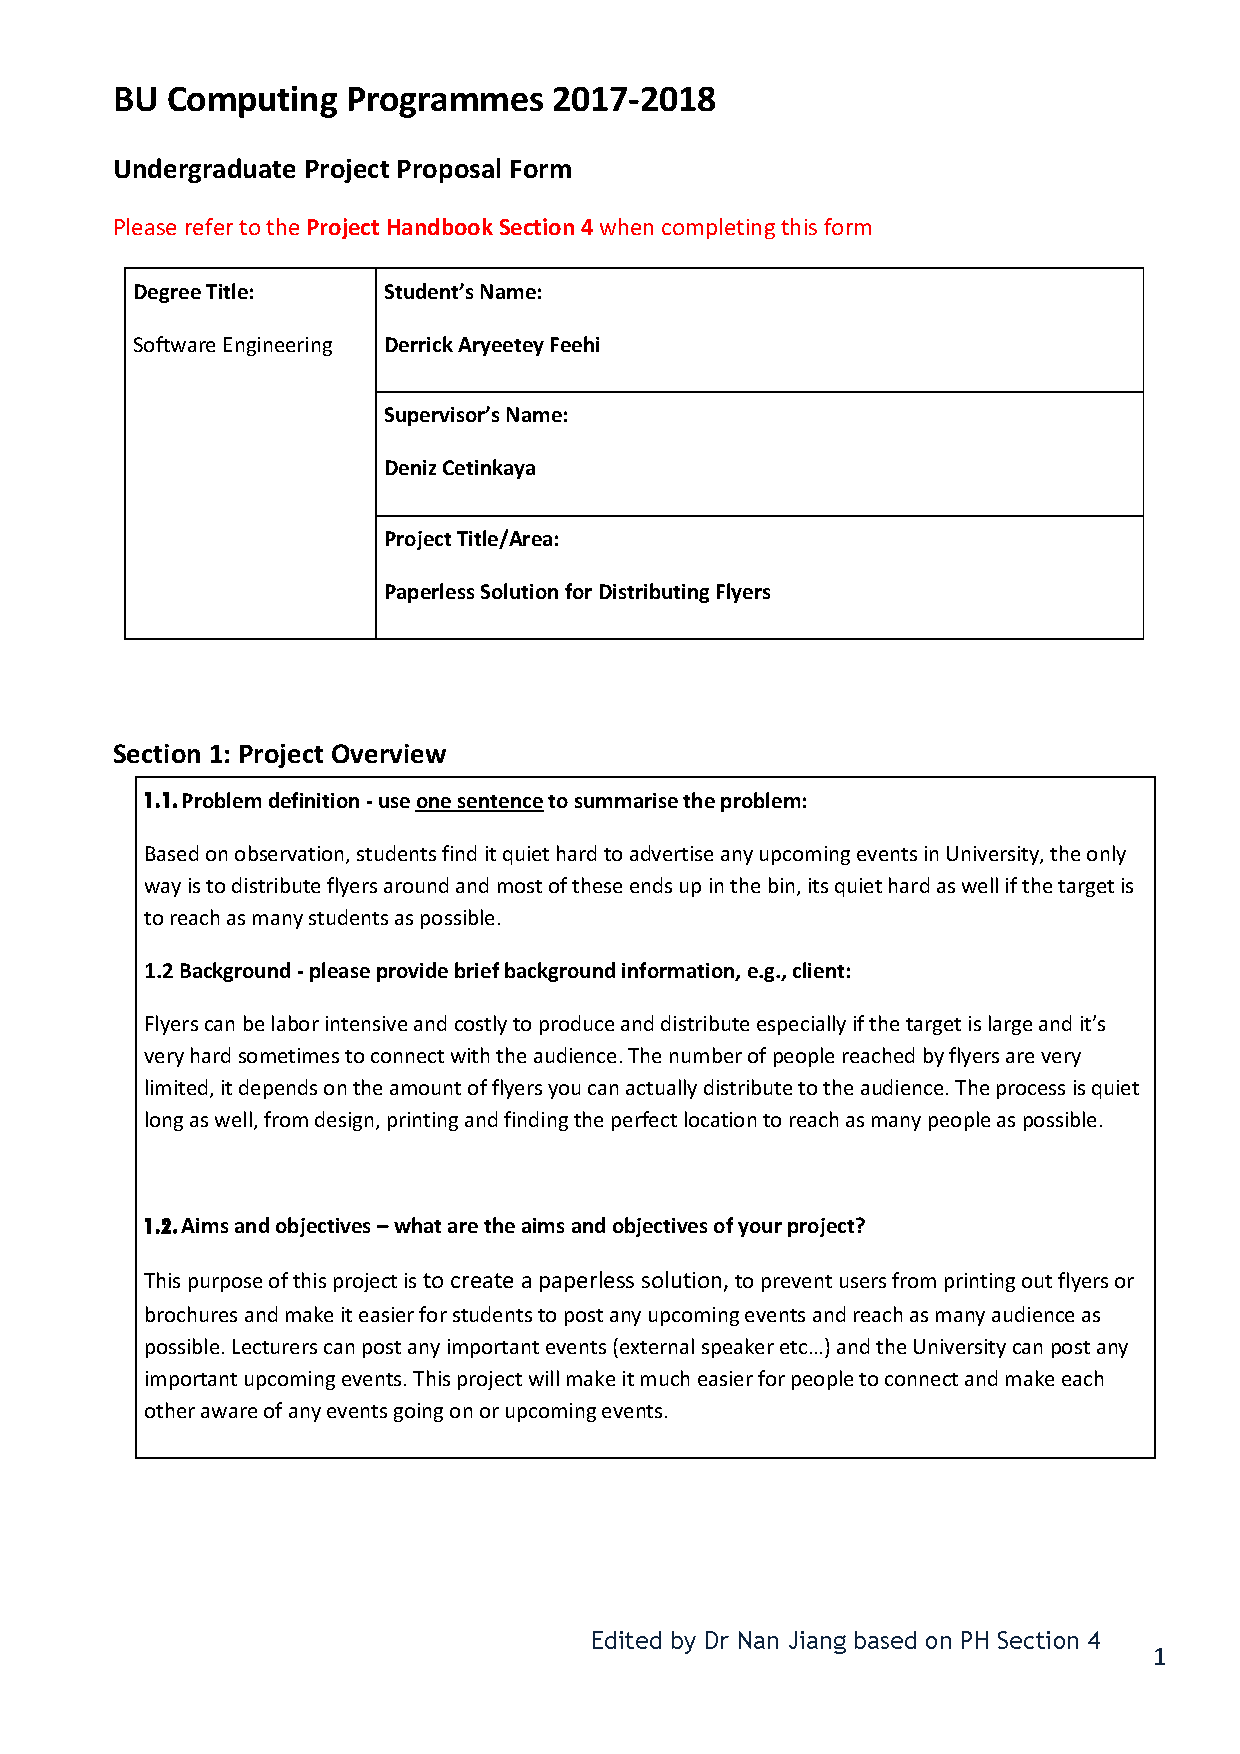
\includepdf[scale=0.85,pages=1,pagecommand=\section{Project Proposal}]{Project_Proposal}
\includepdf[pages=2-5]{Project_Proposal}

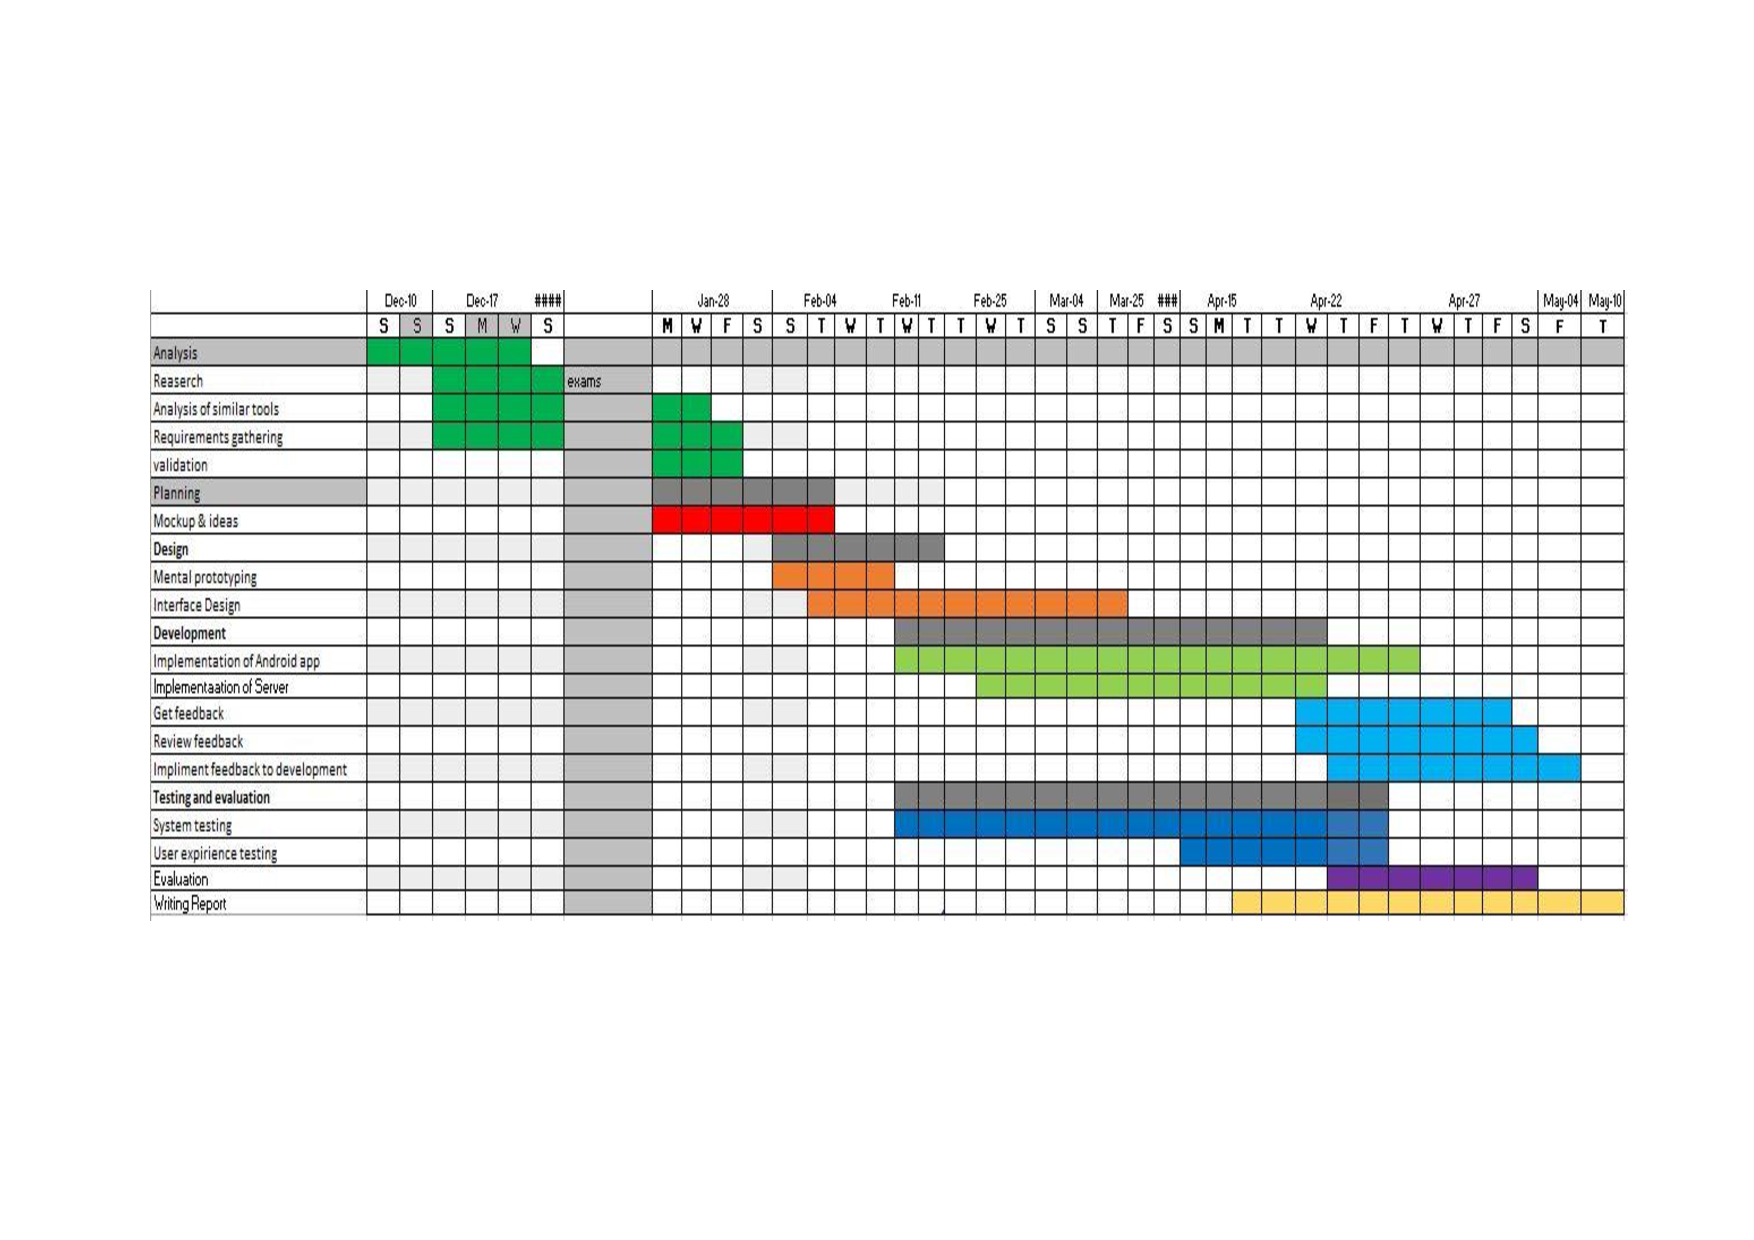
\includepdf[scale=0.85,pages=1,pagecommand=\section{Gantchart} \label{gantchart}]{gantchart}

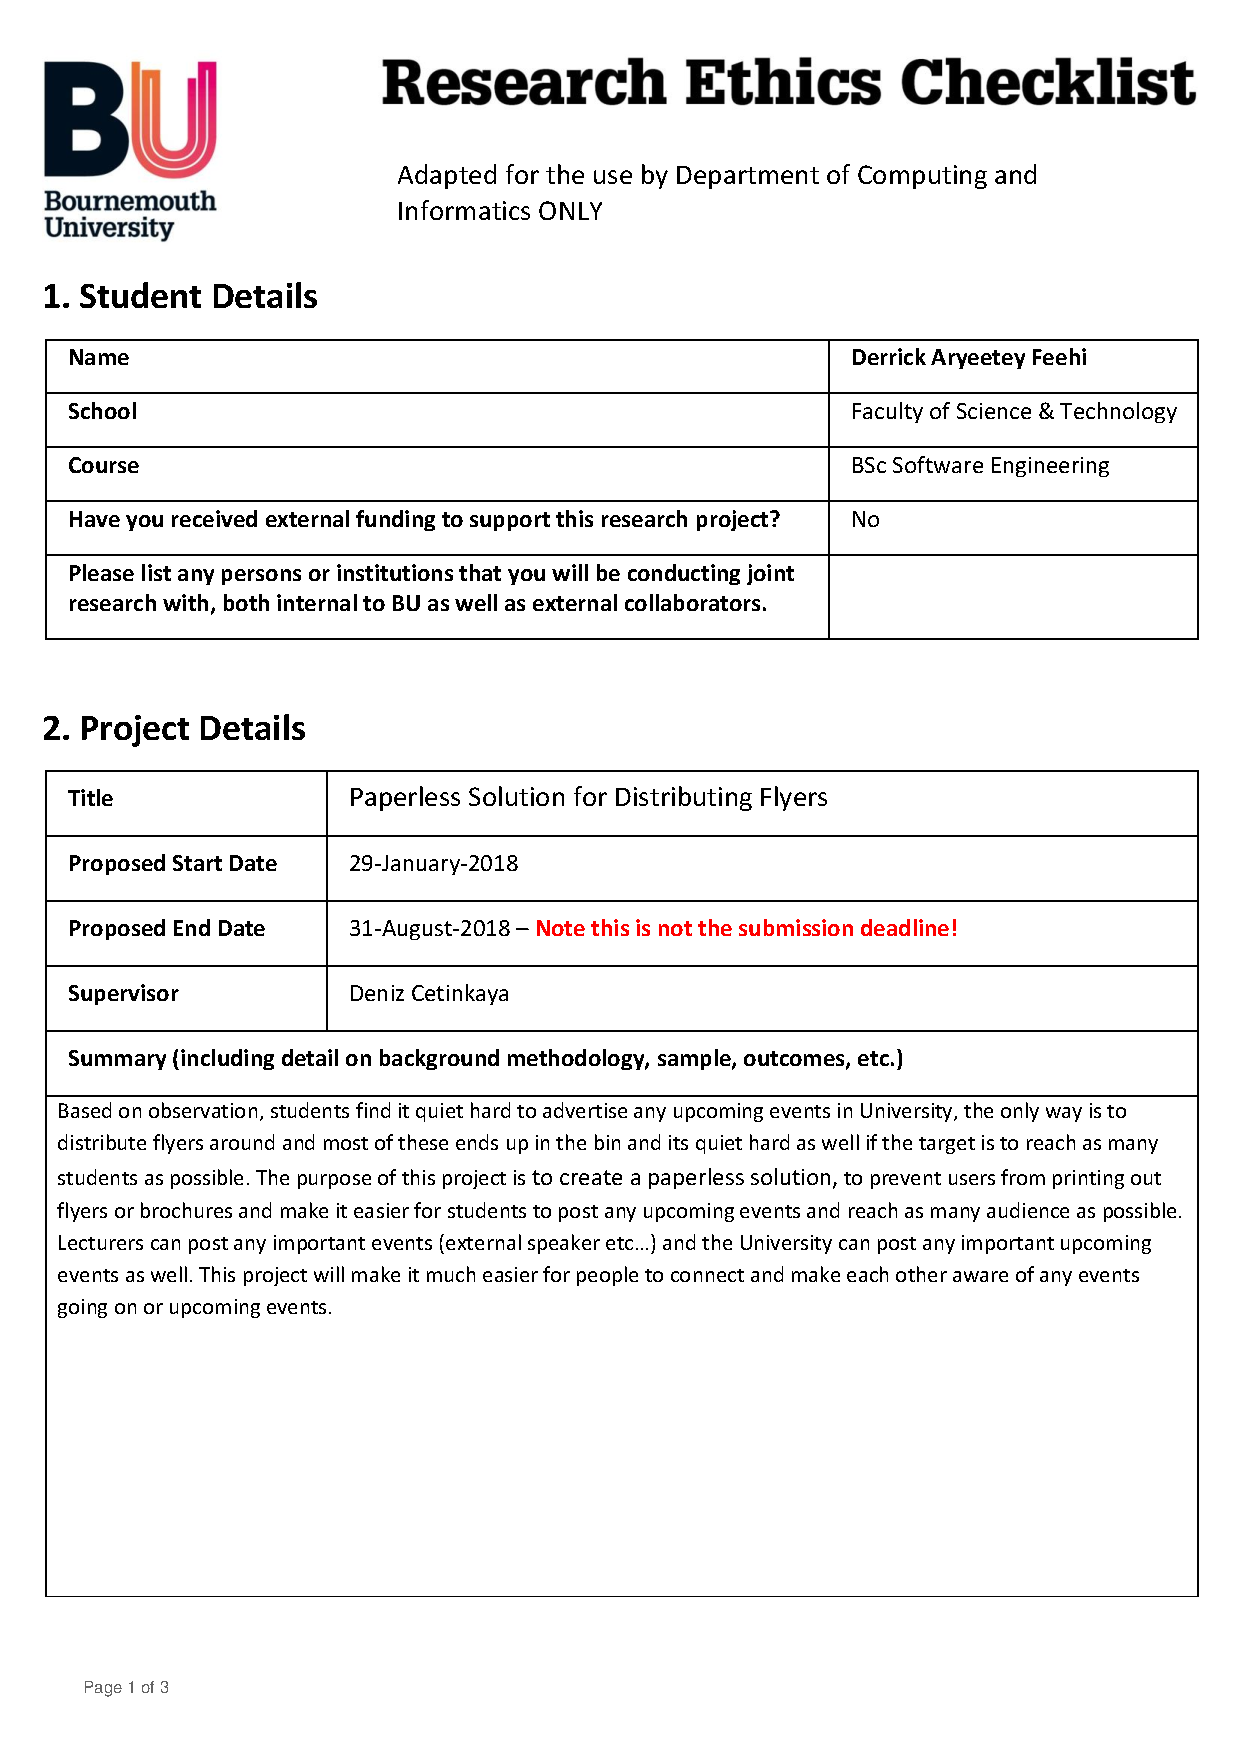
\includepdf[scale=0.85,pages=1,pagecommand=\section{Project Ethics}]{ProjectEthicsForm}
\includepdf[pages=2-6]{ProjectEthicsForm}

\section{Disk Content}
\begin{itemize}
	\item Copy of thesis report in pdf
	\item Database Backup
	\item Android Project Files \& Directory
\end{itemize}



\end{appendices}